\documentclass[tikz,border=10pt]{standalone}
\usetikzlibrary{shapes.geometric, positioning}

\begin{document}
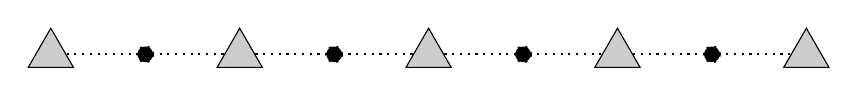
\begin{tikzpicture}[node distance=2cm]

% Define styles for nodes and connections
\tikzset{
    triangle/.style={regular polygon, regular polygon sides=3, draw, fill=black!20},
    dot/.style={circle, inner sep=2pt, draw, fill=black}
}

% Draw the first triangle
\node (triangle1) [triangle] {};

% Draw the second triangle and connect it to the first one
\node (triangle2) [triangle, right=of triangle1] {};
\draw[dotted, thick] (triangle1.east) -- node[dot] {} (triangle2.west);

% Draw the third triangle and connect it to the second one
\node (triangle3) [triangle, right=of triangle2] {};
\draw[dotted, thick] (triangle2.east) -- node[dot] {} (triangle3.west);

% Draw the fourth triangle and connect it to the third one
\node (triangle4) [triangle, right=of triangle3] {};
\draw[dotted, thick] (triangle3.east) -- node[dot] {} (triangle4.west);

% Draw the fifth triangle and connect it to the fourth one
\node (triangle5) [triangle, right=of triangle4] {};
\draw[dotted, thick] (triangle4.east) -- node[dot] {} (triangle5.west);

\end{tikzpicture}
\end{document}